%%% Ne pas modifier jusqu'à la ligne 25
\documentclass[a4paper,12pt]{book}
\usepackage[utf8]{inputenc}
\usepackage[french]{babel}
%%\usepackage{CJK}
\usepackage{yhmath}
\usepackage[left=2cm,right=2cm,top=3cm,bottom=2cm, headheight=1.5cm,headsep=1.5cm]{geometry}
%%\usepackage{CJKutf8}
\usepackage{amsfonts}
\usepackage{mathrsfs}
\usepackage{amsmath,amsfonts,amssymb,dsfont}
\usepackage{graphicx}
\usepackage{subfigure}
\usepackage{enumitem}		%\enumerate-resume
\usepackage[colorlinks=true,unicode={true},hyperindex=false, linkcolor=blue, urlcolor=blue]{hyperref}
\newcommand{\myref}[1]{\ref{#1} page \pageref{#1}}

\addto\captionsfrench{\def\tablename{Tableau}}  %légendes des tableaux
\renewcommand\thesection{\Roman{section}~-~} 
\renewcommand\thesubsection{\Roman{section}.\Alph{subsection}~-~} 
\renewcommand\thesubsubsection{\Roman{section}.\Alph{subsection}.\arabic{subsubsection}~-~} 

\newcommand{\conclusion}[1]{\newline \centerline{\fbox{#1}}}

\setcounter{secnumdepth}{3}
\parindent=0pt

\usepackage{fancyhdr}
\pagestyle{fancy}

\lhead{SJTU-ParisTech} 
%%%%%%%%%%%%%%%%%%%%%%%%%%%%%%%%%%
\chead{TR12}
\rhead{Daniel 518261910024}

\begin{document}
\renewcommand{\labelitemi}{$\blacktriangleright$}
\renewcommand{\labelitemii}{$\bullet$}


\section{Capacité de stockage d'un disque compact}
\subsection{}
\begin{figure}[h]
    \begin{center}
    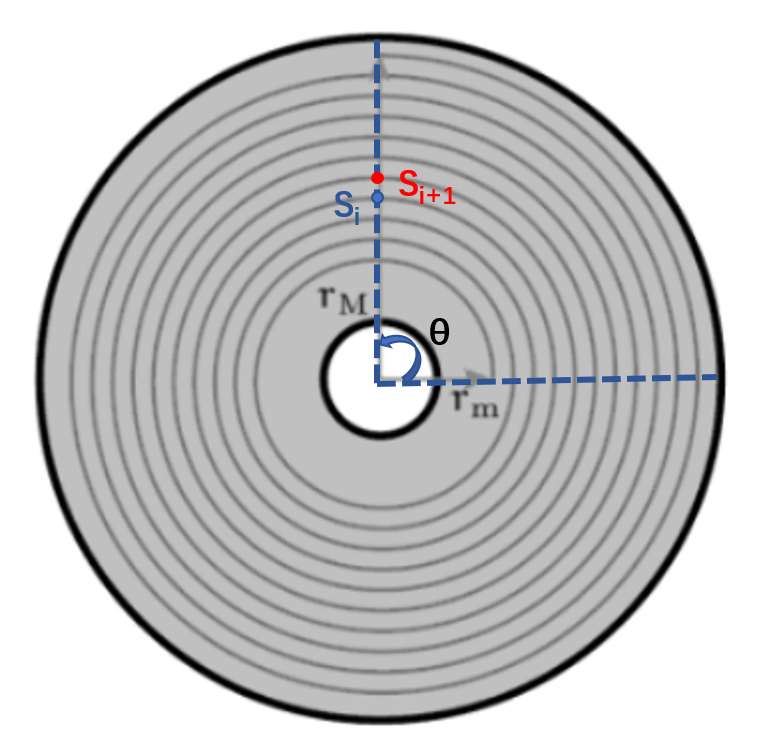
\includegraphics[scale=0.5]{tr12.png}
    \end{center}
    \caption{Figure d'un disque}
\end{figure}
Dans un même axe, la distance entre les deux points adjacents $S_i=(r_i,\theta)$ 
et $S_{i+1}=(r_{i+1},\theta+2\pi)$ est calculée par $r_{i+1}-r_i=\left(r_m+\frac{\theta+2\pi}{2\pi}a\right)-\left(r_m+\frac{\theta}{2\pi}a\right)=a$. 
La distance entre eux est donc une constante indépendante de $\theta$, les fentes sont donc équidistantes. Lorsque la spirale se comporte comme un réseau, 
\fbox{$a$ représente donc le pas du réseau}

\hspace*{\fill} 

\fbox{La spirale fonctionne comme un réseau par réflexion} car les rayons sont réfléchis

\subsection{}
\begin{figure}[h]
    \begin{center}
    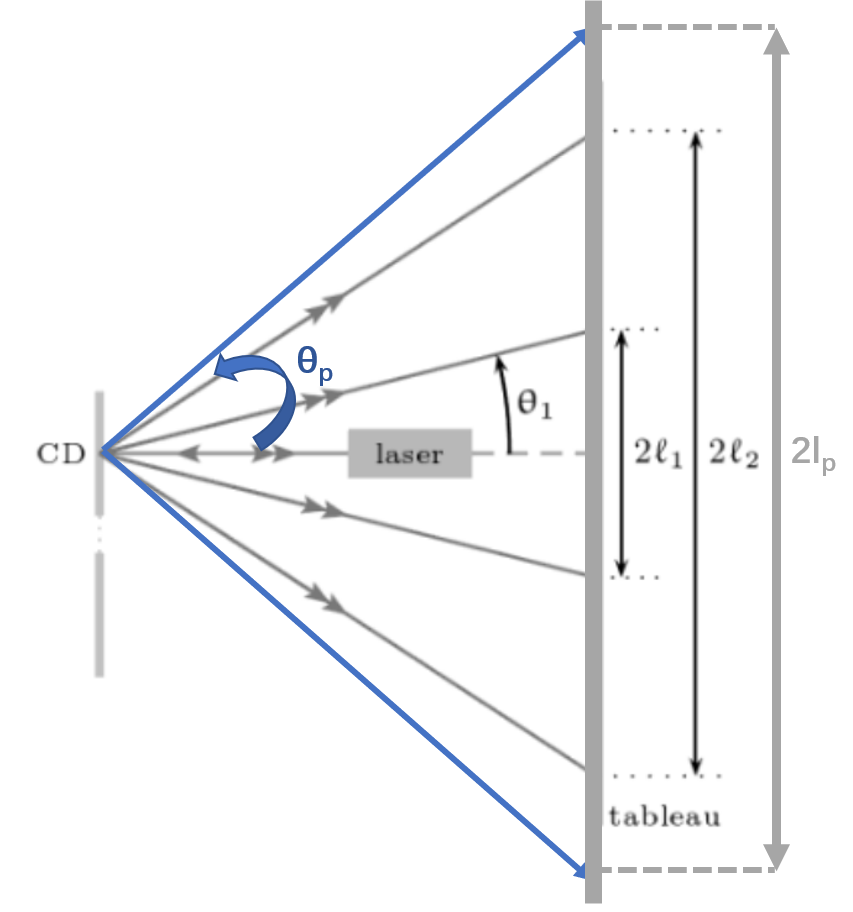
\includegraphics[scale=0.5]{tr122.png}
    \end{center}
    \caption{dispositif expérimental}
\end{figure}
C'est le cas d'un incidence normale, par la formule des réseaux, on a donc $p\lambda_0=a\sin\theta_p$

Par la géométrie, car $\tan \theta_p=\frac{l_p}{D}$, on a donc $\sin\theta_p=\frac{l_p}{l_p^2+D^2}$. 
, on a donc $\boxed{a=p\lambda_0\sqrt{1+\left(\frac{D}{l_p}\right)^2}}$

A.N. Pour $p=1$, on a $a=1*632*10^{-9}*\sqrt{1+\left(\frac{80*10^{-2}}{34*10^{-2}}\right)^2}=1.6*10^{-6}m$, 
pour $p=2$, on

\hspace*{\fill} 

a $a=2*632*10^{-9}*\sqrt{1+\left(\frac{80*10^{-2}}{97.5*10^{-2}}\right)^2}=1.6*10^{-6}m$. 
On a donc $\boxed{a=1.6*10^{-6}m}$, soit $1.6$ 

\hspace*{\fill} 

micromètre, assez fin pour cet expériment.
\subsection{}
Lorsque le rayon $r$ varie entre $r_{min}=r_m$ et $r_{max}=r_M$, l'angle $\theta$ correspondant varie 
entre $\theta_{min}=0$ et $\theta_{max}=\frac{2\pi}{a}(r_M-r_m)$. Par la relation que $dl=r\,d\theta$, 
on a donc 
$$
\int_{l=0}^{l=L}\,dl=\int_{\theta=0}^{\frac{2\pi}{a}(r_M-r_m)} \left(r_m+\frac{a}{2\pi}\theta\right)\,d\theta
$$
où $L$ est la longueur de la piste. 
On a donc $L=\boxed{\frac{\pi}{a}r_M^2-\frac{\pi}{a}r_m^2}$. 

\hspace*{\fill} 

A.N. $\boxed{L=\frac{\pi}{1.6*10^{-6}}((58*10^{-3})^2-(22*10^{-3})^2)=5.6*10^3\,m}$, soit $5.6\,km$ 



\subsection{}
On a la distance entre deux bits d'information le long de la piste est $d=\frac{1}{2}a=0.8*10^{-6}m$, 
donc le nombre de bits $N=\frac{L}{d}=\frac{5.6*10^3}{0.8*10^{-6}}=7*10^{9}\,bits$, soit \fbox{$875$ Mo}.
Il est un peu petit, donc on n'utilise pas souvent les disques pour stocker les données aujourd'hui. 


\end{document}